%package list
\documentclass[]{article}
\usepackage[top=3cm, bottom=3cm, outer=3cm, inner=3cm]{geometry}
\usepackage{graphicx}
\usepackage{url}
%\usepackage{cite}
\usepackage{hyperref}
\usepackage{array}
%\usepackage{multicol}
\newcolumntype{x}[1]{>{\centering\arraybackslash\hspace{0pt}}p{#1}}
\usepackage{natbib}
\usepackage{pdfpages}
\usepackage[export]{adjustbox}
% \usepackage{multirow}
\usepackage[T1]{fontenc}
\usepackage{imakeidx}
% Imagenes de costado
% \usepackage{wrapfig}
% \usepackage{graphicx}

% Modificar URLs
\usepackage{hyperref}
\hypersetup{
    colorlinks=true,
    linkcolor=black,
    filecolor=magenta,      
    urlcolor=blue,
    pdftitle={Overleaf Example},
    pdfpagemode=FullScreen,
    }

\urlstyle{same}


\usepackage[normalem]{ulem}
\useunder{\uline}{\ul}{}

\usepackage[newfloat]{minted}
\usepackage{caption}

\newenvironment{code}{\captionsetup{type=listing}}{}
\SetupFloatingEnvironment{listing}{name=Source Code}

% codigo fuente
\usepackage{listings}
\usepackage{color, colortbl}
\definecolor{dkgreen}{rgb}{0,0.6,0}
\definecolor{gray}{rgb}{0.5,0.5,0.5}
\definecolor{mauve}{rgb}{0.58,0,0.82}
\definecolor{codebackground}{rgb}{0.95, 0.95, 0.92}
\definecolor{tablebackground}{rgb}{0.0, 0.45, 0.63}
\lstset{frame=tb,
	language=bash,
	aboveskip=3mm,
	belowskip=3mm,
	showstringspaces=false,
	columns=flexible,
	basicstyle={\small\ttfamily},
	numbers=none,
	numberstyle=\tiny\color{gray},
	keywordstyle=\color{blue},
	commentstyle=\color{dkgreen},
	stringstyle=\color{mauve},
	breaklines=true,
	breakatwhitespace=true,
	tabsize=3,
	backgroundcolor= \color{codebackground},
}

%%%%%%%%%%%%%%%%%%%%%%%%%%%%%%%%%%%%%%%%%%%%%%%%%%%%%%%%%%%%%%%%%%%%%%%%%%%%
%%%%%%%%%%%%%%%%%%%%%%%%%%%%%%%%%%%%%%%%%%%%%%%%%%%%%%%%%%%%%%%%%%%%%%%%%%%%
\newcommand{\csemail}{pramirezs@ulasalle.edu.pe}
\newcommand{\csdocente}{MSc. Maribel Molina Barriga}
\newcommand{\cscurso}{Sistemas Operativos}
\newcommand{\csuniversidad}{Universidad La Salle}
\newcommand{\csescuela}{Escuela Profesional de Ingeniería de Software}
\newcommand{\cspracnr}{03}
\newcommand{\cstema}{Compilacion en C y C++ en Linux}
%%%%%%%%%%%%%%%%%%%%%%%%%%%%%%%%%%%%%%%%%%%%%%%%%%%%%%%%%%%%%%%%%%%%%%%%%%%%
%%%%%%%%%%%%%%%%%%%%%%%%%%%%%%%%%%%%%%%%%%%%%%%%%%%%%%%%%%%%%%%%%%%%%%%%%%%%


\usepackage[english,spanish]{babel}
\usepackage[utf8]{inputenc}
\AtBeginDocument{\selectlanguage{spanish}}
\renewcommand{\figurename}{Figura}
\renewcommand{\refname}{Referencias}
\renewcommand{\tablename}{Tabla} %esto no funciona cuando se usa babel
\AtBeginDocument{%
	\renewcommand\tablename{Tabla}
}

\usepackage{fancyhdr}
\pagestyle{fancy}
\fancyhf{}
\setlength{\headheight}{30pt}
\renewcommand{\headrulewidth}{1pt}
\renewcommand{\footrulewidth}{1pt}
\fancyhead[L]{\raisebox{-0.2\height}{
\includegraphics[width=3cm]{logo_ulasalle.png}}}
\fancyhead[C]{}
\fancyhead[R]{\fontsize{7}{7}\selectfont	\csuniversidad \\ \csescuela \\ \textbf{\cscurso} }
\fancyfoot[L]{}
\fancyfoot[C]{Sistemas Operativos}
\fancyfoot[R]{Página \thepage}



\begin{document}

	\vspace*{10px}
	
	\begin{center}	
		\fontsize{17}{17} \textbf{Practica \cspracnr}
	\end{center}
	%\centerline{\textbf{\underline{\Large Título: Informe de revisión del estado del arte}}}
	%\vspace*{0.5cm}
	

\renewcommand{\arraystretch}{1.5}
\begin{table}[h]
	\begin{tabular}{|x{4.7cm}|x{4.8cm}|x{4.8cm}|}
		\hline 
		\textbf{DOCENTE} & \textbf{CARRERA}  & \textbf{CURSO}   \\
		\hline 
		\csdocente & \csescuela & \cscurso    \\
		\hline 
	\end{tabular}
\end{table}	

\begin{table}[h]
	\begin{tabular}{|x{4.7cm}|x{4.8cm}|x{4.8cm}|}
		\hline 
		\textbf{GRUPO} & \textbf{TEMA}  & \textbf{DURACIÓN}   \\
		\hline 
		\ 6 & \cstema & 5 horas   \\
		\hline 
	\end{tabular}
\end{table}
\renewcommand{\arraystretch}{1} 
	\section*{Integrantes}
	 	\begin{itemize}
            \item José Carlos Machaca Vera
	 		\item Jhosep Alonso Mollapaza Morocco
	 		\item Patrick Andres Ramirez Santos
	 \end{itemize}
 
	\tableofcontents
\newpage

\section{Ejercicios propuestos}
Se deberá de probar, compilar y ejecutar los siguientes códigos:
\subsection{Ejercicio 1}
Se crea un archivo Cmake para facilitar la compilacion y ejecucion 
del codigo, este se presenta a continuacion, y que se puede utilizar 
con los siguientes comandos desde el directorio con los archivos:

\begin{minted}{bash}
	$ mkdir cmake-build-debug/
	$ cd cmake-build-debug/
	$ cmake .. # Buscar el archivo CMakeLists.txt en el directorio superior
	$ make # Compilar el proyecto
	$ ./E1 # Ejecutar el proyecto
\end{minted}

\begin{code}
	\captionof{listing}{Contenidos Makefile}
	\inputminted{cmake}{../E1/CMakeLists.txt}
\end{code}

\subsubsection*{proceso.cpp}
Este código crea un proceso hijo que imprime un mensaje en pantalla.
\begin{code}
	\captionof{listing}{Contenidos Makefile}
	\inputminted{c}{../E1/proceso.c}
\end{code}


\subsubsection*{ejemplo.cpp}
Este código utiliza polimorfismo para detectar el tipo de un objeto e imprimir
una funcion especifica en base a ello:
\begin{code}
	\captionof{listing}{Contenidos Makefile}
	\inputminted{c}{../E1/ejemplo.cpp}
\end{code}

\subsection{Ejercicio 2}
Este código recibe 2 argumentos vía línea de comandos, el primero es un 
número de segundos y el segundo es un mensaje, el código espera el tiempo
definido por el primer argumento y luego imprime el mensaje en pantalla 
de forma indefinida.
\begin{code}
	\captionof{listing}{E2/main.cpp}
	\inputminted{cpp}{../E2/main.cpp}
\end{code}

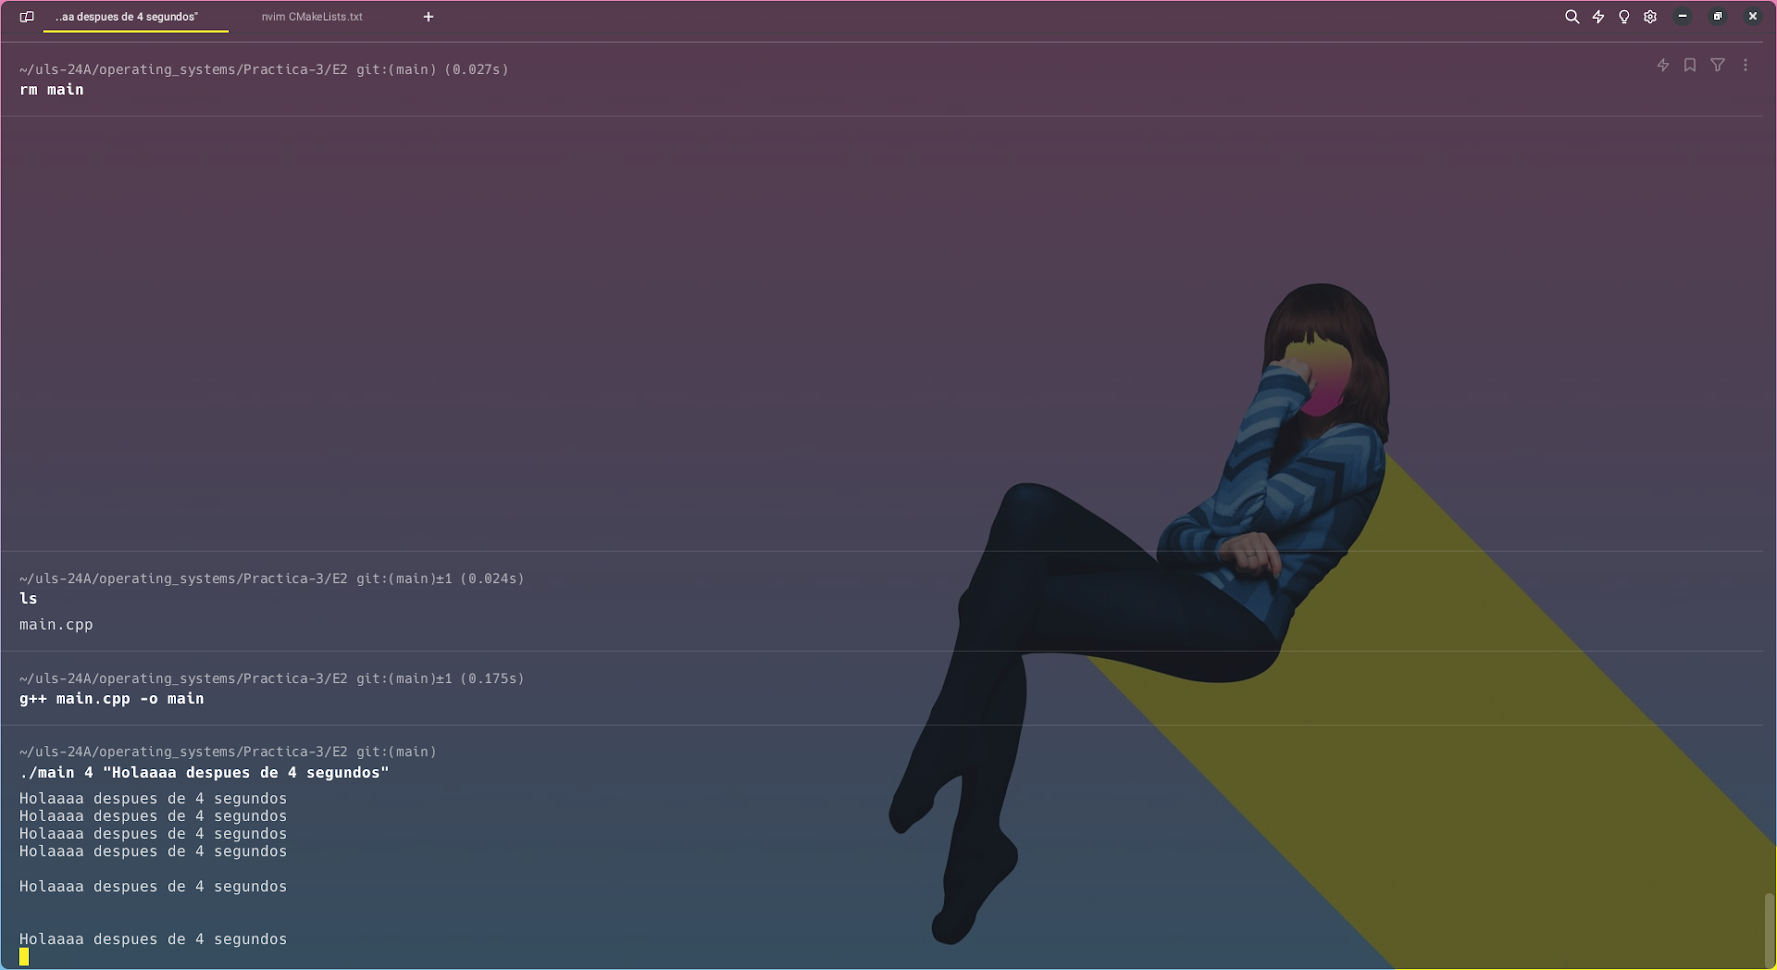
\includegraphics[scale=0.3,trim={0 0 20cm 20cm},clip]{e2-out.png}  

\subsection{Ejercicio 3}
En este ejercicio se utiliza un Makefile para compilar el archivo mensaje.c
y los archivos que este requiere para ejecutarse, para ejecutarlo se deben 
seguir los siguientes comandos, luego se muestra el contenido del Makefile:
\begin{minted}{bash}
	$ make # Compilar el proyecto con el makefile
	$ ./mensaje # Ejecutar el proyecto
\end{minted}

\begin{code}
	\captionof{listing}{E3/Makefile}
	\label{code:c-code}
	\inputminted{Makefile}{../E3/Makefile}
\end{code}
		
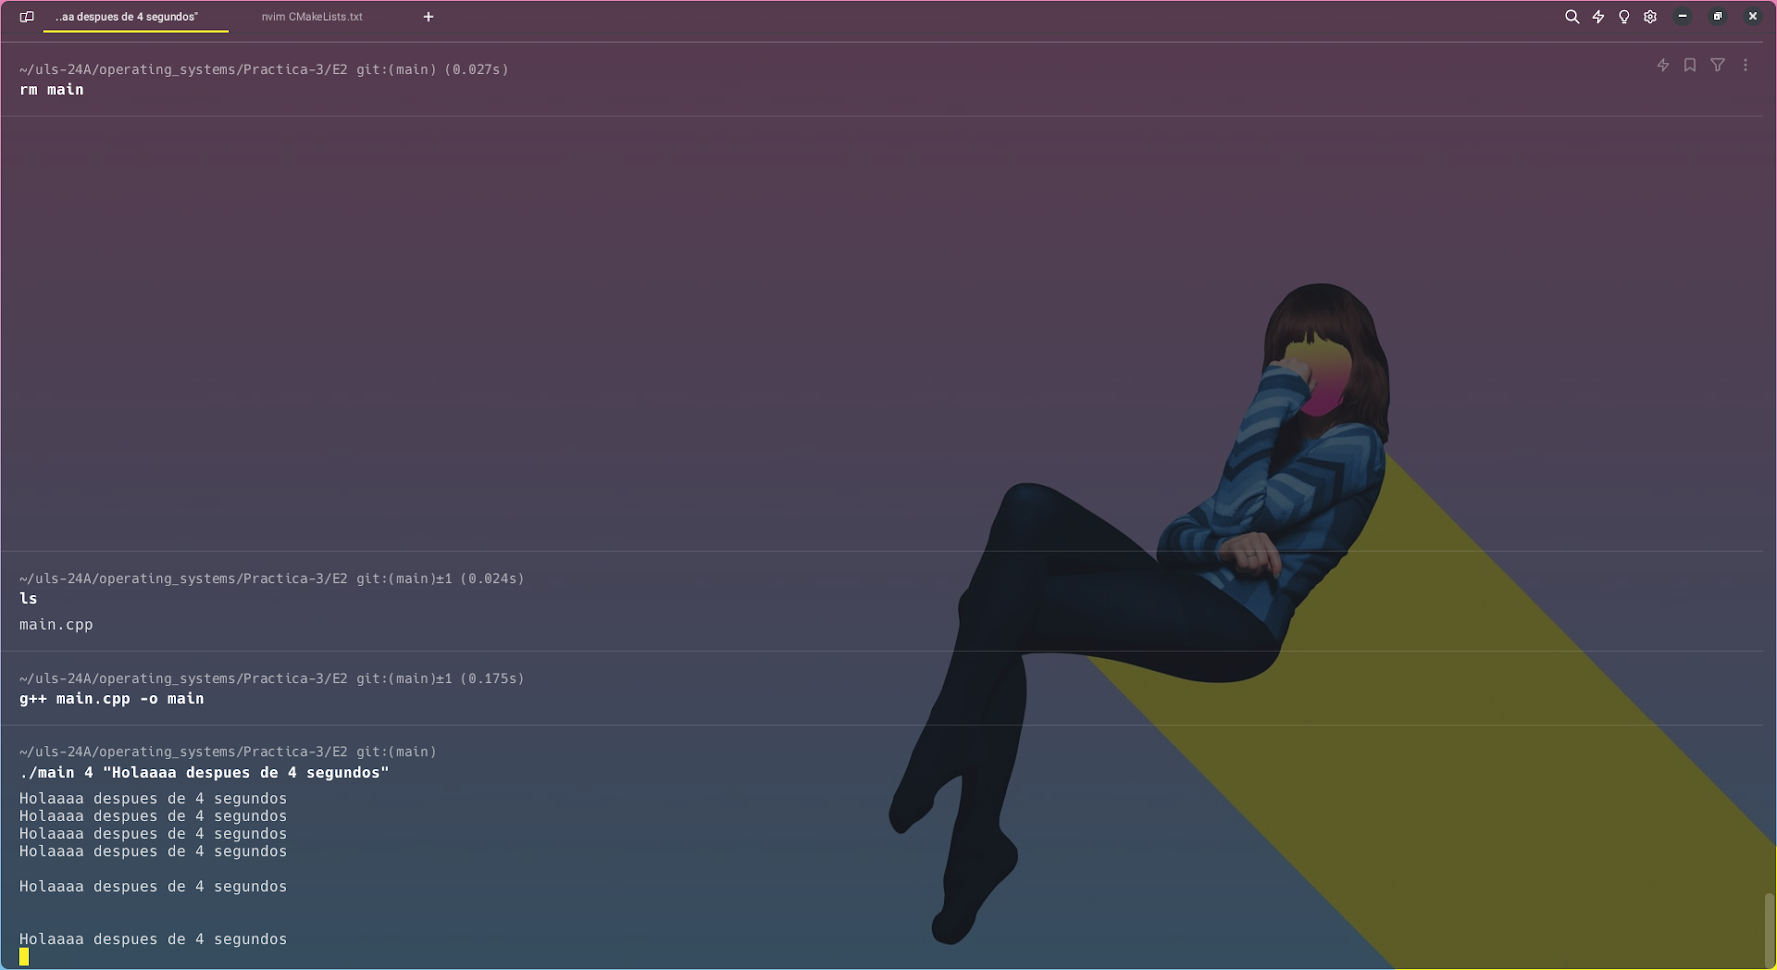
\includegraphics[scale=0.3,trim={0 0 20cm 20cm},clip]{e2-out.png}  


\section{Cuestionario}


\renewcommand{\listlistingname}{Indice Source Code}
\listoflistings

% \section{Cuadrilla KEKW}
%    \begin{tabular}{cc}
%        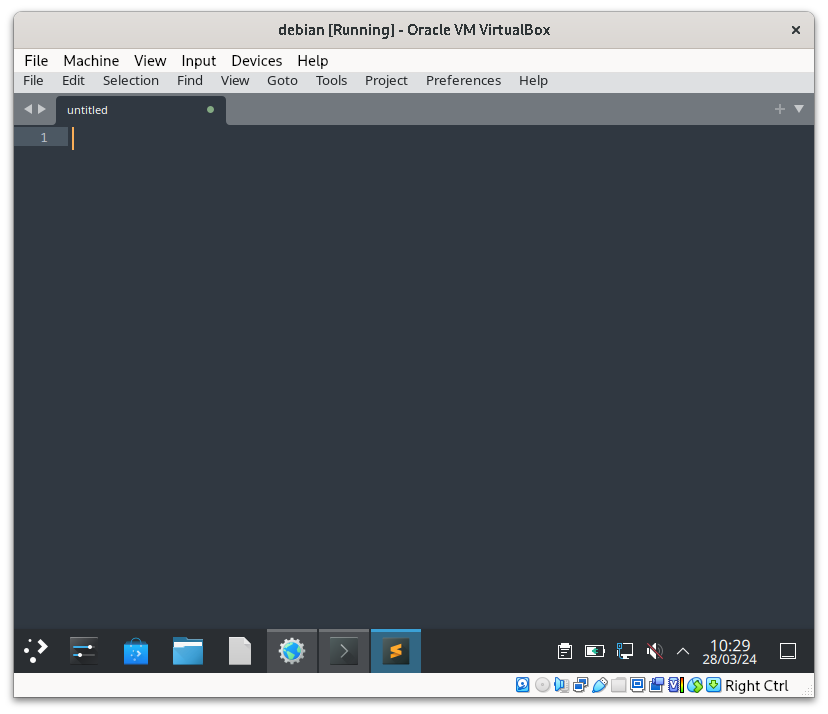
\includegraphics[width=.4\linewidth,valign=m]{capturas_paquetes/sublime.png} & 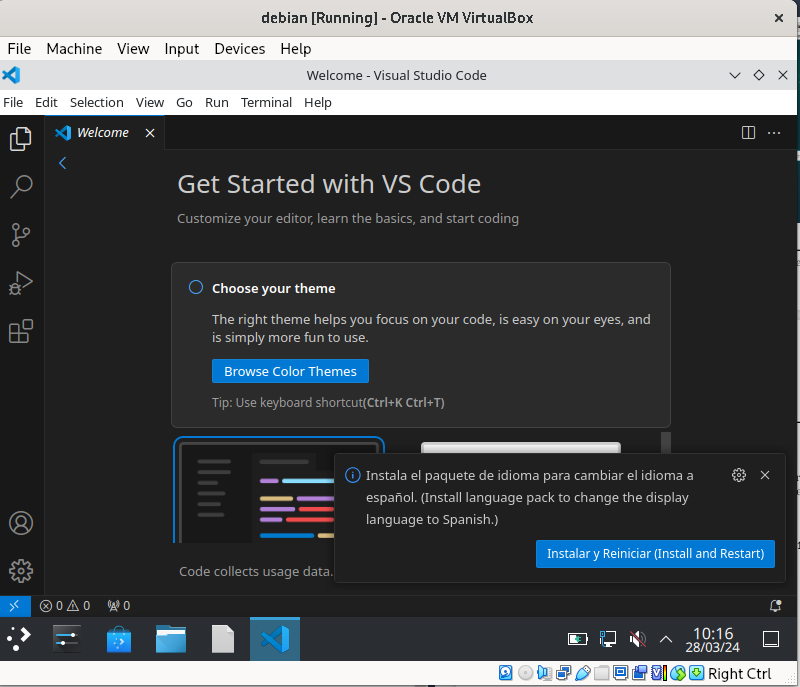
\includegraphics[width=.4\linewidth,valign=m]{capturas_paquetes/vscode.png} \\
%        Sublime & VS Code \\
%        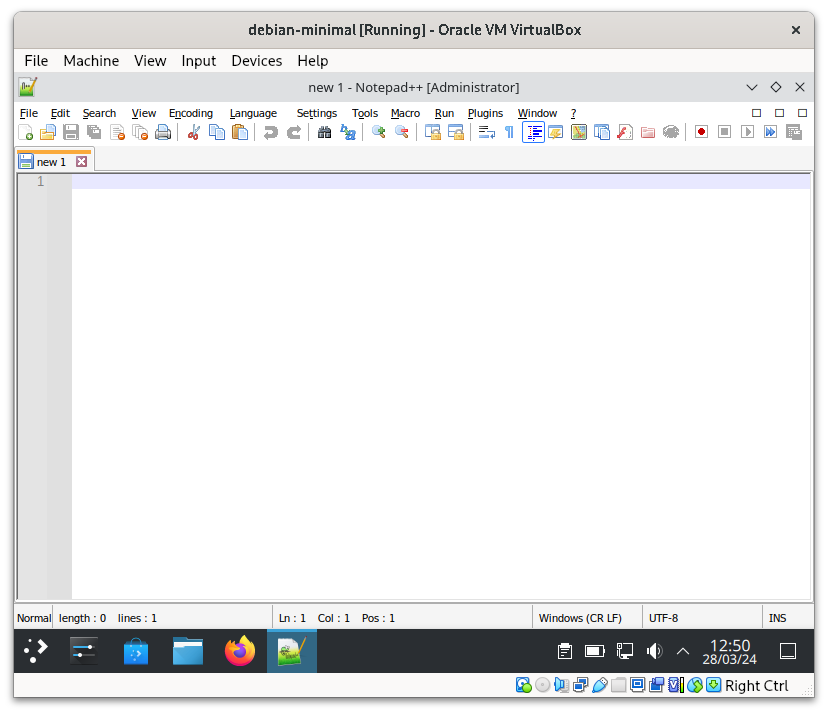
\includegraphics[width=.4\linewidth,valign=m]{capturas_paquetes/notepad.png} & 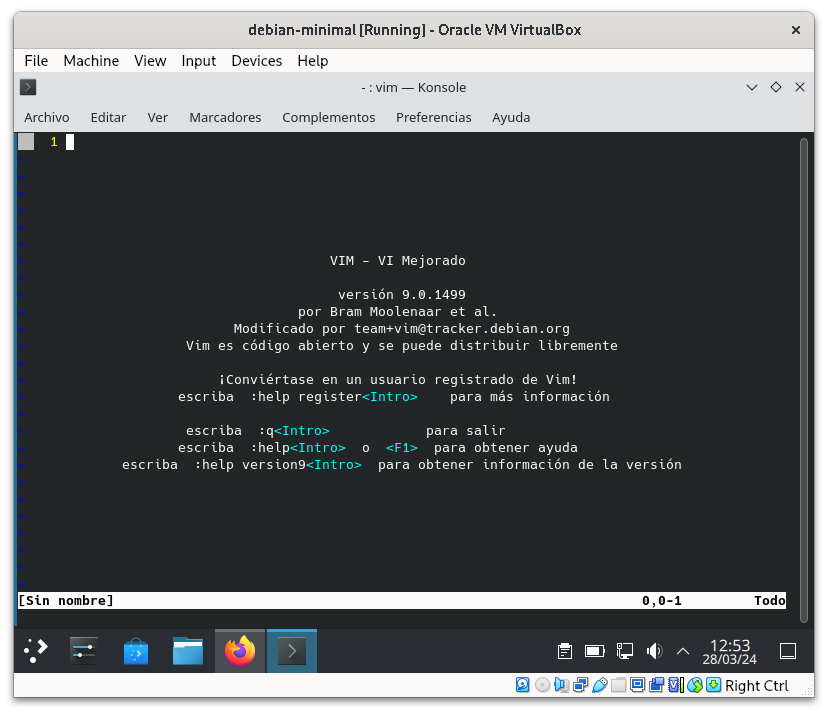
\includegraphics[width=.4\linewidth,valign=m]{capturas_paquetes/vim.png} \\
%        Notepad++ & Vim \\
%    \end{tabular}

	%\clearpage
	%\bibliographystyle{apalike}
	%\bibliographystyle{IEEEtranN}
	%\bibliography{bibliography}
		
	
\end{document}
